\problemname{Hoppers}
\noindent
Joshua has built a factory in minecraft, which consists of a grid where each cell contains a so-called hopper.
A hopper can store an item within it, and points towards another hopper that is located either directly above, below, to the left or to the right of it.
Once per second, each hopper pushes the item they have inside themselves to the hopper they are pointing at if they have an item inside.
Sometimes this can lead to a hopper having more than one item inside simultaneously.
This obviously doesn't work, as all the items pushed into the hopper that second are destroyed.

Joshua wants a stable factory without a lot of collisions.
He therefore gives you a proposal on how the items should be placed and how the factory should look, and now wants to know
for each item if it will collide or keep cycling endlessly in the factory.
For all the items that collide, he also wants to know where the collision occurred so he can then update his design.
Write a program to help him!

\begin{figure}[h]
  \centering
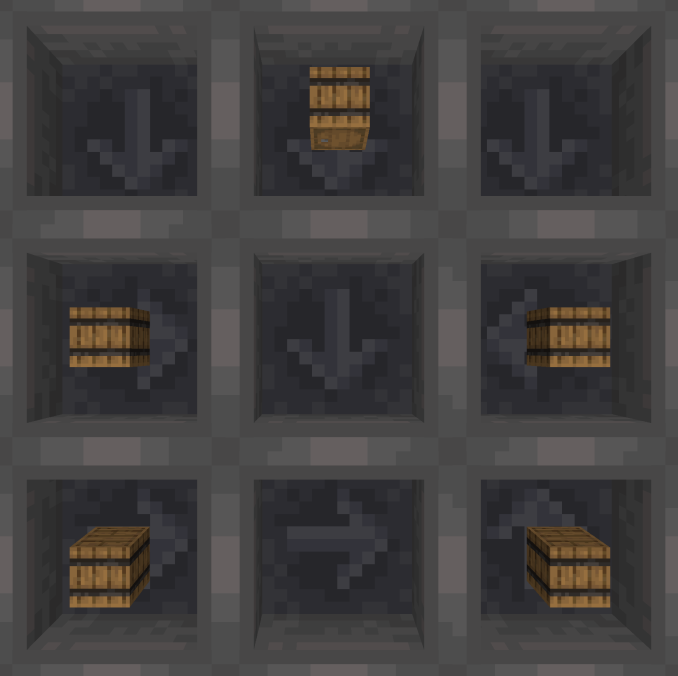
\includegraphics[width=0.25\textwidth]{hoppers_t0.png}
\quad
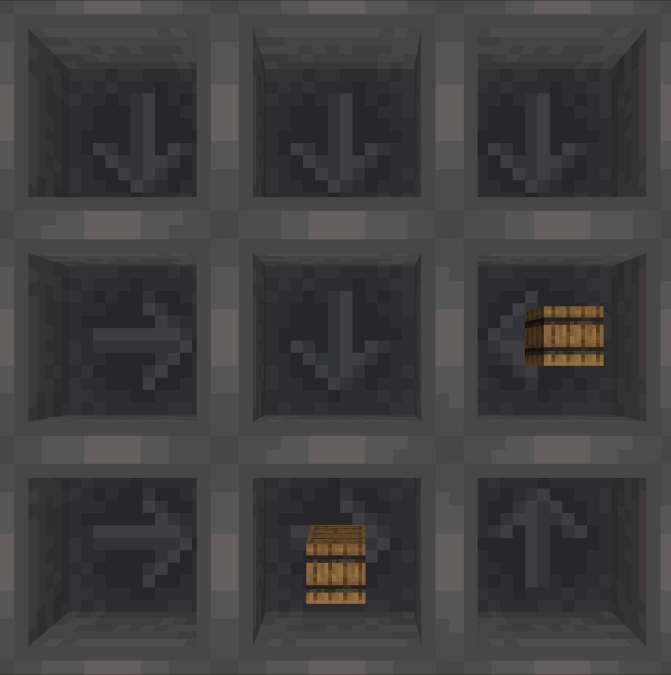
\includegraphics[width=0.25\textwidth]{hoppers_t1.png}
  \caption{The factory in sample 1 before it has started and after one second. Note that three items collided
  in the middle square.}
  \label{fig:hoppers_t0}
\end{figure}


\section*{Input}
\noindent
The first line contains the integers $R, C$ $R, C$ ($2 \le R \cdot C \le 10^6$), $N$ ($1 \le N \le 10^5$),
the number of rows and columns of the grid, and the number of items in the proposal.
 
The following $R$ rows describe the layout of the factory. Each of these rows consists of a string of $C$
characters.
Each character in the grid indicates the direction the hopper in that square is pointing towards.
The characters will either be '\texttt{v}' (down), '\texttt{<}' (left), '\texttt{\^}' (up), or '\texttt{>}' (right).
It is guaranteed that each hopper points to another hopper.

Then follows $N$ rows, each containing two integers $P_r$ ($0 \leq P_r \leq R-1$) and $P_c$ ($0 \leq P_c \leq C-1$),
the row and column where the $i$th item starts. No hopper initially contains two or more items.

\section*{Output}
\noindent
For each item in the same order as in the input, 
print a line with "\texttt{cycle}" if the item never collides with anything, or "$r$ $c$" if it
collides with something in the hopper at row $r$ and column $c$ ($0$-indexed).

\section*{Scoring}
Your solution will be tested on a set of test groups, each worth a number of points. 
Each test group contains a set of test cases. 
To get the points for a test group you need to solve all test cases in the test group.

\noindent
\begin{tabular}{| l | l | p{12cm} |}
  \hline
  \textbf{Group} & \textbf{Point value} & \textbf{Constraints} \\ \hline
  $1$    & $10$      & $R \cdot C \le 1000, N \le 1000$ \\ \hline
  $2$    & $35$      & $N \le 1000$ \\ \hline
  $3$    & $15$      & If a hopper is part of a cycle, then at most one other hopper points towards it. \\ \hline
  $4$    & $25$      & No hopper points upwards. \\ \hline
  $5$    & $15$      & No additional constraints. \\ \hline
\end{tabular}
